% ECE 592 Homework 3 (Track B) report.
% Compile from this directory:  pdflatex report.tex  (run twice for refs)
% Figures are read from ../analysis/out/ (regenerate with the scripts in analysis/).
% On Overleaf: upload rob_prf.png, tlb.png, tlb_pmu.png and enclave.png to the project root
% or to a figures/ folder; both are on the search path below.
\documentclass[11pt]{article}
\usepackage[margin=1in]{geometry}
\usepackage[T1]{fontenc}
\usepackage{lmodern}
\usepackage{graphicx}
\usepackage{booktabs}
\usepackage{tabularx}
\usepackage{listings}
\usepackage{xcolor}
\usepackage{caption}
\usepackage{enumitem}
\usepackage[hidelinks]{hyperref}

\graphicspath{{../analysis/out/}{figures/}{./}}
\setlist{nosep,leftmargin=*}
\lstset{
  basicstyle=\ttfamily\footnotesize,
  columns=fullflexible,
  keepspaces=true,
  frame=single,
  framerule=0.4pt,
  rulecolor=\color{gray!60},
  backgroundcolor=\color{gray!6},
  commentstyle=\color{gray!70!black},
  showstringspaces=false,
  xleftmargin=0.5em,
  xrightmargin=0.5em,
}
\newcommand{\up}{\texttt{upgrade}}
\newcommand{\sk}{\texttt{skylark}}
\newcommand{\file}[1]{\texttt{\detokenize{#1}}}

\title{ECE 592 Homework 3 --- Microarchitecture Reverse Engineering\\[0.3em]
\large Track B: individual work, AI use disclosed}
\author{Nicholas Ngo}
\date{November 4, 2026}

\begin{document}
\maketitle

\section*{Selected questions}

\begin{center}
\begin{tabular}{clr}
\toprule
Q\# & Question & Points \\
\midrule
4 & Reverse engineer the ROB size & 30 \\
5 & Reverse engineer the physical register file size; identify the register class & 35 \\
6 & Reverse engineer the number of TLB levels and the size of each level & 35 \\
8 & Measure the cost of a TLB miss & 10 \\
9 & Compare TLB behavior across supported page sizes & 10 \\
\midrule
 & \textbf{Total} & \textbf{120} \\
\bottomrule
\end{tabular}
\end{center}

Q4 and Q5 share one experiment (Section~\ref{sec:rob}); Q6, Q8 and Q9 share
another (Section~\ref{sec:tlb}). Every experiment was run on two course
machines, \up{} (Intel) and \sk{} (AMD), and the results are presented side by
side. The enclave comparison ran on a third, SGX-enabled machine
(Section~\ref{sec:enclave}). Source code, raw data, plotting scripts and reproduction instructions
are in the accompanying ZIP (Appendix~\ref{app:repro}); AI use is recorded in
\file{AI_LOG.md}.

\paragraph{Convention.} Throughout, \emph{measured} values come from my
experiments and \emph{published} values come from the cited sources, which are
mostly secondary (such as WikiChip) rather than vendor manuals. The two are
always in separate table columns.

% ---------------------------------------------------------------------------
\section{Machines and access limitations}
\label{sec:machines}

\begin{table}[h]
\centering
\small
\begin{tabularx}{\linewidth}{@{}lXX@{}}
\toprule
 & \up{} & \sk{} \\
\midrule
CPU & Intel Core i7-8700 (6 cores, 12 threads) & AMD EPYC 7532 (2 sockets $\times$ 32 cores, 128 threads) \\
Microarchitecture & Coffee Lake (Skylake family) & Zen 2 (Rome), family 23 model 49 \\
Microcode & \texttt{0xfa} & \texttt{0x830107d} \\
OS kernel & Linux 6.8 (Ubuntu 22.04) & Linux 5.14 (RHEL 9) \\
Timer used & TSC, 3.19 GHz & TSC, 2.40 GHz, \emph{and} core cycles via perf \\
Core clock during runs & unknown (\texttt{powersave} governor, turbo up to 4.6 GHz) & $\approx$1.49 GHz (1.61 TSC ticks per core cycle, \texttt{userspace} governor) \\
perf counters & \textbf{No} (\texttt{perf\_event\_paranoid}=4) & Yes (\texttt{perf\_event\_paranoid}=2) \\
2 MiB pages & Yes, transparent huge pages & Yes, transparent huge pages \\
1 GiB pages & \textbf{No} (no hugetlbfs pool; needs root) & \textbf{No} (no hugetlbfs pool; needs root) \\
Enclave & \textbf{No}: SGX not enabled (no \texttt{/dev/sgx*}) & \textbf{No}: AMD has no SGX; SEV disabled by BIOS \\
\bottomrule
\end{tabularx}
\caption{Machines. Full records: \file{data/<host>/machine_info.txt}. A third
machine with SGX, \texttt{artemisia}, was used only for the enclave
comparison (Section~\ref{sec:enclave}).}
\label{tab:machines}
\end{table}

\paragraph{Units.} On \up{} only the TSC is available, and the core clock
during a run is unknown (turbo), so \up{} results are in TSC ticks or ns.
On \sk{} core cycles are read with \texttt{perf\_event\_open}, so \sk{}
results are in core cycles. Because the two machines also ran at very
different clocks (up to 4.6 GHz vs.\ 1.49 GHz), absolute times are not
comparable across machines; step \emph{positions} (entry counts) are.

\paragraph{Common setup.} Each experiment pins itself to one idle logical
CPU (CPU~2 unless stated) and reports the median of 5--9 repetitions per
point. Timed code is hand-written or generated assembly so the compiler
cannot reorder or remove it.

% ---------------------------------------------------------------------------
\section{Q4 and Q5: ROB and physical register files}
\label{sec:rob}

\subsection{Method}

I use the two-miss technique of Henry Wong (2013). Each loop iteration
performs two \emph{independent} loads that miss in every cache level (two
random pointer chases through 256~MiB buffers), separated by $N$ filler
instructions:

\begin{lstlisting}[language={[x86masm]Assembler},caption={Generated kernel for the integer filler (annotated excerpt of \file{build/rob_prf_kernels.S}, produced by \file{exp/rob_prf/gen_kernels.py}).}]
k_int_N:
    mov  rax, rdi          ; chain A pointer
    mov  rcx, rsi          ; chain B pointer (independent of A)
1:  mov  rax, [rax]        ; load A: misses to DRAM
    add  r8, r8            ; N filler instructions
    add  r9, r9            ;   (rotate r8-r11, rsi, rdi)
    ...
    mov  rcx, [rcx]        ; load B: misses to DRAM
    add  r8, r8            ; N more fillers
    ...
    dec  rdx
    jnz  1b
\end{lstlisting}

\textbf{What is tested.} While load A, the $N$ fillers and load B all fit in
the out-of-order window, the two misses overlap and an iteration costs about
one memory latency. When the fillers exhaust some back-end resource, load B
cannot be dispatched until load A retires, and the iteration cost jumps to
about two memory latencies. The $N$ at which the jump happens measures the
resource that ran out first. The filler type chooses that resource:

\begin{center}
\small
\begin{tabular}{lll}
\toprule
Filler & Consumes per instruction & Measures \\
\midrule
\texttt{nop} & 1 ROB entry, no register & ROB size (Q4) \\
\texttt{add r64, r64} & 1 ROB entry + 1 integer physical register & integer PRF (Q5) \\
\texttt{addps xmm, xmm} & 1 ROB entry + 1 vector/FP physical register & vector PRF (Q5) \\
alternating int / vec & half the demand on each register file & register class (Q5) \\
\bottomrule
\end{tabular}
\end{center}

\textbf{How the results support the conclusions.}
\begin{itemize}
\item \emph{ROB}: with \texttt{nop} the window holds load A, $N$ fillers and
  load B, so the step at $N$ gives ROB $\approx N + 2$.
\item \emph{PRF}: \texttt{nop} writes no register, so if the \texttt{add}
  or \texttt{addps} curve steps at a \emph{smaller} $N$, a register file,
  not the ROB, is the limit. The committed values of the 16 architectural
  registers of that class must also stay in physical registers, so the step
  gives a lower bound: PRF $\gtrsim N + 16$.
\item \emph{Register class}: if integer and vector registers came from one
  shared pool, the alternating filler would step at the same $N$ as the
  single-class fillers. If they are separate pools, each pool sees only
  half the demand, and the alternating curve steps much later (at the ROB
  limit).
\end{itemize}
The sweep covers $N = 0, 4, \dots, 640$. The vector registers are zeroed
before the loop so \texttt{addps} never produces denormals (which would
trigger microcode assists).

\subsection{Results}

\begin{figure}[h]
\centering
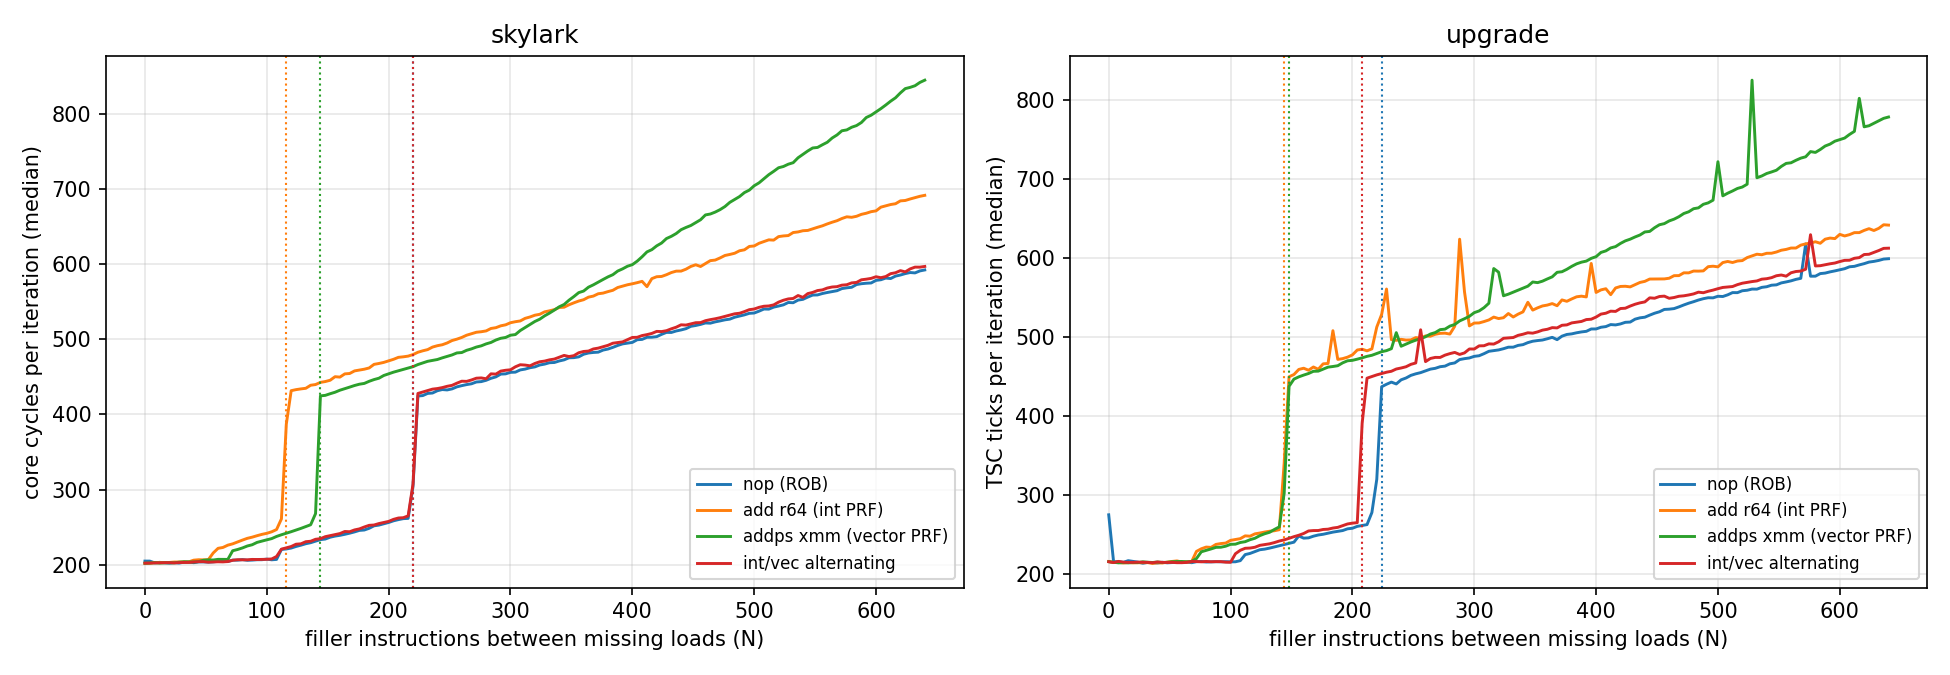
\includegraphics[width=\linewidth]{rob_prf.png}
\caption{Cycles (\sk, core cycles) or TSC ticks (\up) per iteration vs.\
filler count $N$; dotted lines mark the detected steps. Median of 5--9
repetitions per point. Data: \file{data/<host>/rob_prf/}.}
\label{fig:rob}
\end{figure}

\begin{table}[h]
\centering
\small
\begin{tabular}{lcc|cc}
\toprule
 & \multicolumn{2}{c|}{\textbf{Measured} step at $N$} & \multicolumn{2}{c}{\textbf{Published}} \\
Filler & \up{} (3 runs) & \sk{} (3 runs) & Coffee Lake & Zen 2 \\
\midrule
\texttt{nop} (ROB) & 220, 220, 224 & 224, 220, 220 & 224 & 224 \\
\texttt{add} (int PRF) & 148, 144, 144 & 116, 116, 116 & 180 & 180 \\
\texttt{addps} (vec PRF) & 148, 144, 148 & 144, 144, 144 & 168 & 160 \\
alternating & 208, 208, 208 & 220, 220, 220 & --- & --- \\
\bottomrule
\end{tabular}
\caption{Step positions. Sweep resolution is 4, so a step reported at $N$
lies in $(N-4, N]$. \sk{} runs 1--2 on CPU~2 (socket 0), run 3 on CPU~40
(socket 1). Published values (Coffee Lake uses the Skylake core):
Skylake ROB and integer PRF~\cite{wc-skl,arxiv-skx}, vector PRF~\cite{arxiv-skx,wp-snc};
Zen 2~\cite{wc-zen2}.}
\label{tab:rob}
\end{table}

\subsection{Interpretation}

\paragraph{Q4, ROB size.} Both machines step at $N = 220$--$224$, giving a
measured ROB of about $222$--$226$ entries, consistent with the published 224
on both. The two microarchitectures, from different vendors, converge on the
same ROB size.

\paragraph{Q5, PRF size.} On both machines the register-writing fillers step
well before \texttt{nop}, so register files, not the ROB, bound the window.
\begin{itemize}
\item \sk{} vector: step 144, so PRF $\gtrsim 160$, matching the published 160 exactly.
\item \up{} vector: step 144--148, so PRF $\gtrsim 160$--$164$, against a published 168.
\item \up{} integer: step 144--148, so PRF $\gtrsim 160$--$164$, against a published 180.
\item \sk{} integer: step 116, so PRF $\gtrsim 132$, against a published 180.
\end{itemize}
The lower bound is close for the vector files and \up{} integer, but \sk{}'s
integer step is 64 below the published size (36 on \up). Something else holds
integer physical registers while the loop runs. Candidates are the loop
counter and the two chase pointers, and on Zen 2 possibly flag results
(\texttt{add} also writes the flags). I have not isolated this; it is listed
as an open question (Section~\ref{sec:open}).

\paragraph{Q5, register class.} The alternating filler steps at 208
(\up) and 220 (\sk), next to the ROB limit and far beyond the
single-class steps (116--148). If integer and vector results shared one
pool, alternating would step at the same $N$ as the single-class fillers.
Therefore, on both machines, \textbf{integer and vector/FP physical
registers are separate register files}. On \sk{} the alternating curve lies
directly on the \texttt{nop} curve: splitting the demand removes the
register limit entirely. On \up{} it steps about 12 earlier than
\texttt{nop}. At $N = 208$ each file sees only about 104 allocations, far
below the single-class steps, so two separate pools do not explain this gap;
it is listed as an open question (Section~\ref{sec:open}).

\paragraph{Differences between machines.} Same ROB size; the vector PRF
behaves similarly; the integer PRF limit is reached much earlier on Zen 2.
Repeatability is high: all \sk{} runs, on both sockets, agree within the
sweep resolution of 4.

% ---------------------------------------------------------------------------
\section{Q6, Q8 and Q9: TLB levels, miss cost and page sizes}
\label{sec:tlb}

\subsection{Method}

A chain of dependent loads touches one 64-byte slot in each of $P$ pages in
a random order, and $P$ is swept. Each time $P$ exceeds the reach of a TLB
level, the time per access steps up (Q6). The height of each step is the
cost of that kind of miss (Q8). Running the sweep with 4~KiB and 2~MiB pages
gives Q9.

\begin{lstlisting}[language={[x86masm]Assembler},caption={Timed loop (\file{exp/tlb/tlb_chase.S}). Each load's address depends on the previous load's value, so accesses are serialized and the time per access is load latency plus any TLB-miss penalty.}]
1:  mov  rax, [rdi + rcx*8]   ; next slot address (sequential, prefetchable)
    add  rax, rdx             ; + previous value (always 0): creates dependency
    mov  rdx, [rax]           ; the measured access
    inc  rcx
    cmp  rcx, rsi             ; wrap around after P pages
    jne  2f
    xor  ecx, ecx
2:  dec  r9
    jnz  1b
\end{lstlisting}

\textbf{Separating TLB effects from cache effects.} Cache reverse engineering
is out of scope, but caches also produce steps as $P$ grows, so three access
patterns are compared:

\begin{center}
\small
\begin{tabularx}{\linewidth}{@{}lX@{}}
\toprule
Pattern & Construction and purpose \\
\midrule
\texttt{alias} (4~KiB only) & $P$ virtual pages all mapped to \emph{one} physical page (a \texttt{memfd} mapped $P$ times). The data is always L1-resident; only translations vary. Intended as the pure TLB signal. \\
\texttt{private} & One slot in each of $P$ separate physical pages. TLB + cache effects. \\
\texttt{dense} & $P$ slots in consecutive lines of a few huge pages: the same data footprint with almost no TLB demand. Control for the cache-only cost. \\
\bottomrule
\end{tabularx}
\end{center}

The slot offset rotates through the page (page $i$ uses line $i$ mod
lines-per-page), spreading slots across cache sets. For 2~MiB pages
aliasing is not possible, so the TLB signal is \texttt{private} $-$
\texttt{dense}. Transparent huge pages are best effort, so every 2~MiB page
is verified (via \file{/proc/self/smaps_rollup}) before use, and pages that
fall back to 4~KiB are discarded.

\begin{lstlisting}[language=C,caption={Building the \texttt{alias} pattern (\file{exp/tlb/main.c}).}]
int fd = memfd_create("hw3_tlb_alias", 0);   /* one 4 KiB physical page */
ftruncate(fd, SZ_4K);
for (size_t i = 0; i < pages; i++)            /* map it at P virtual pages */
    mmap(base + i * SZ_4K, SZ_4K, PROT_READ | PROT_WRITE,
         MAP_SHARED | MAP_FIXED | MAP_POPULATE, fd, 0);
\end{lstlisting}

\textbf{Hardware-counter confirmation (\sk{} only).} Because perf is
available on \sk, the driver can also read AMD DTLB events around every
timed repetition (\texttt{build/tlb -e}, \file{scripts/tlb_pmu.sh}): L1 DTLB
misses (PMC 0x45, all umasks), L1 misses that hit or miss the L2 TLB (per
page size), coalesced-page hits, and data-side page-table walks (PMC 0x46).
This gives a timing-independent check that each step is a TLB step. With the
NMI watchdog and the cycle counter each holding one of the six core
counters, at most four events are counted, and each row records whether the
kernel multiplexed a counter; no row in the data was multiplexed.

\begin{lstlisting}[language=C,caption={Event counts per access read around each timed repetition (\file{exp/tlb/main.c}).}]
for (int k = 0; k < c->nev; k++) e0[k] = raw_read(c->efd[k], &muxed);
uint64_t t0 = tsc_now();
tlb_chase(c->addrs, pages, total);
uint64_t t1 = tsc_now();
for (int k = 0; k < c->nev; k++) e1[k] = raw_read(c->efd[k], &muxed);
/* written as (e1[k] - e0[k]) / total, plus a pmu_muxed flag */
\end{lstlisting}

\subsection{Results}

\begin{figure}[p]
\centering
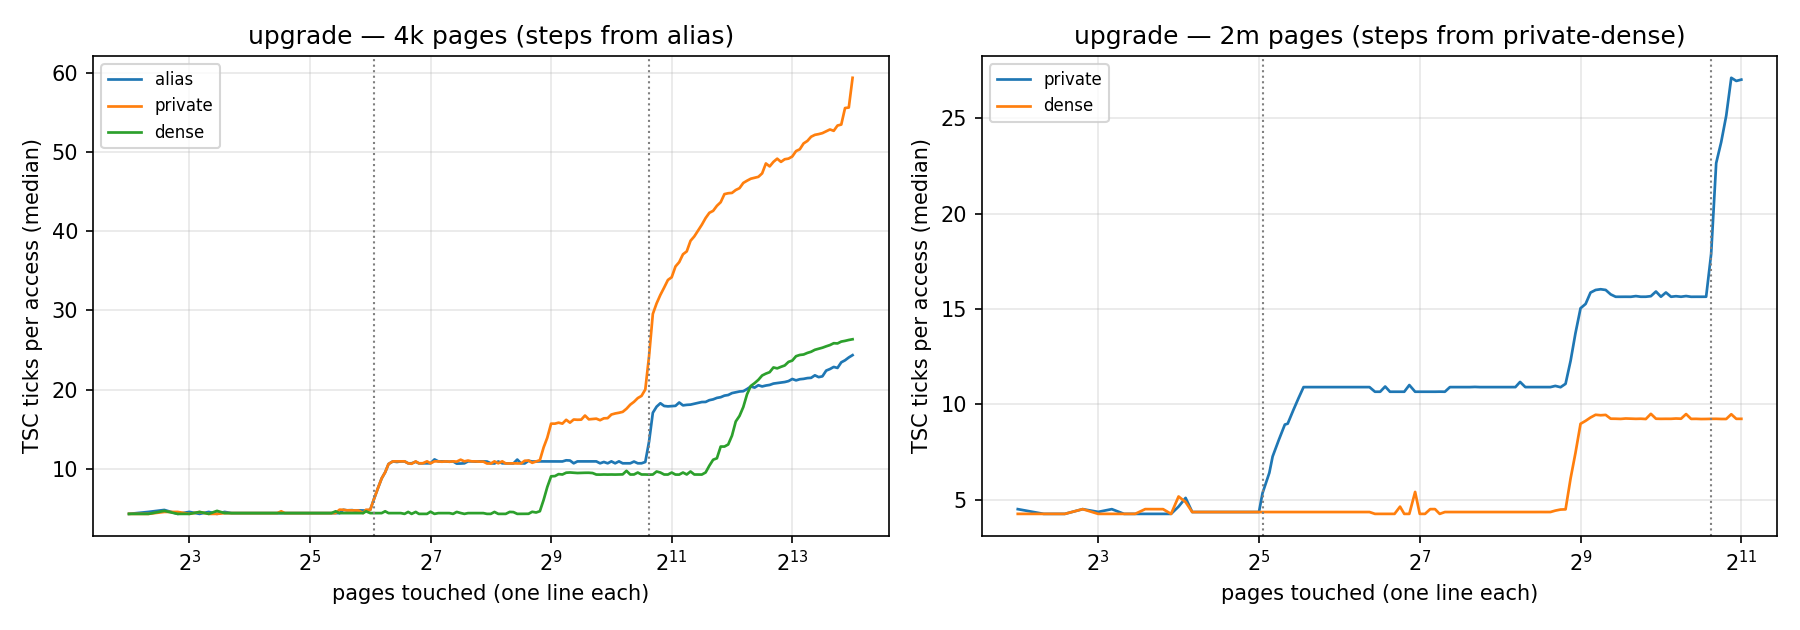
\includegraphics[width=\linewidth]{tlb.png}
\caption{TSC ticks per access vs.\ pages touched, both machines and page
sizes (\up{} bottom, \sk{} top). Dotted lines mark steps found by the
automatic detector. The detector misses the gradual \sk{} 4~KiB L2 ramp;
Figure~\ref{fig:pmu} shows it with counters.}
\label{fig:tlb}
\vspace{1em}
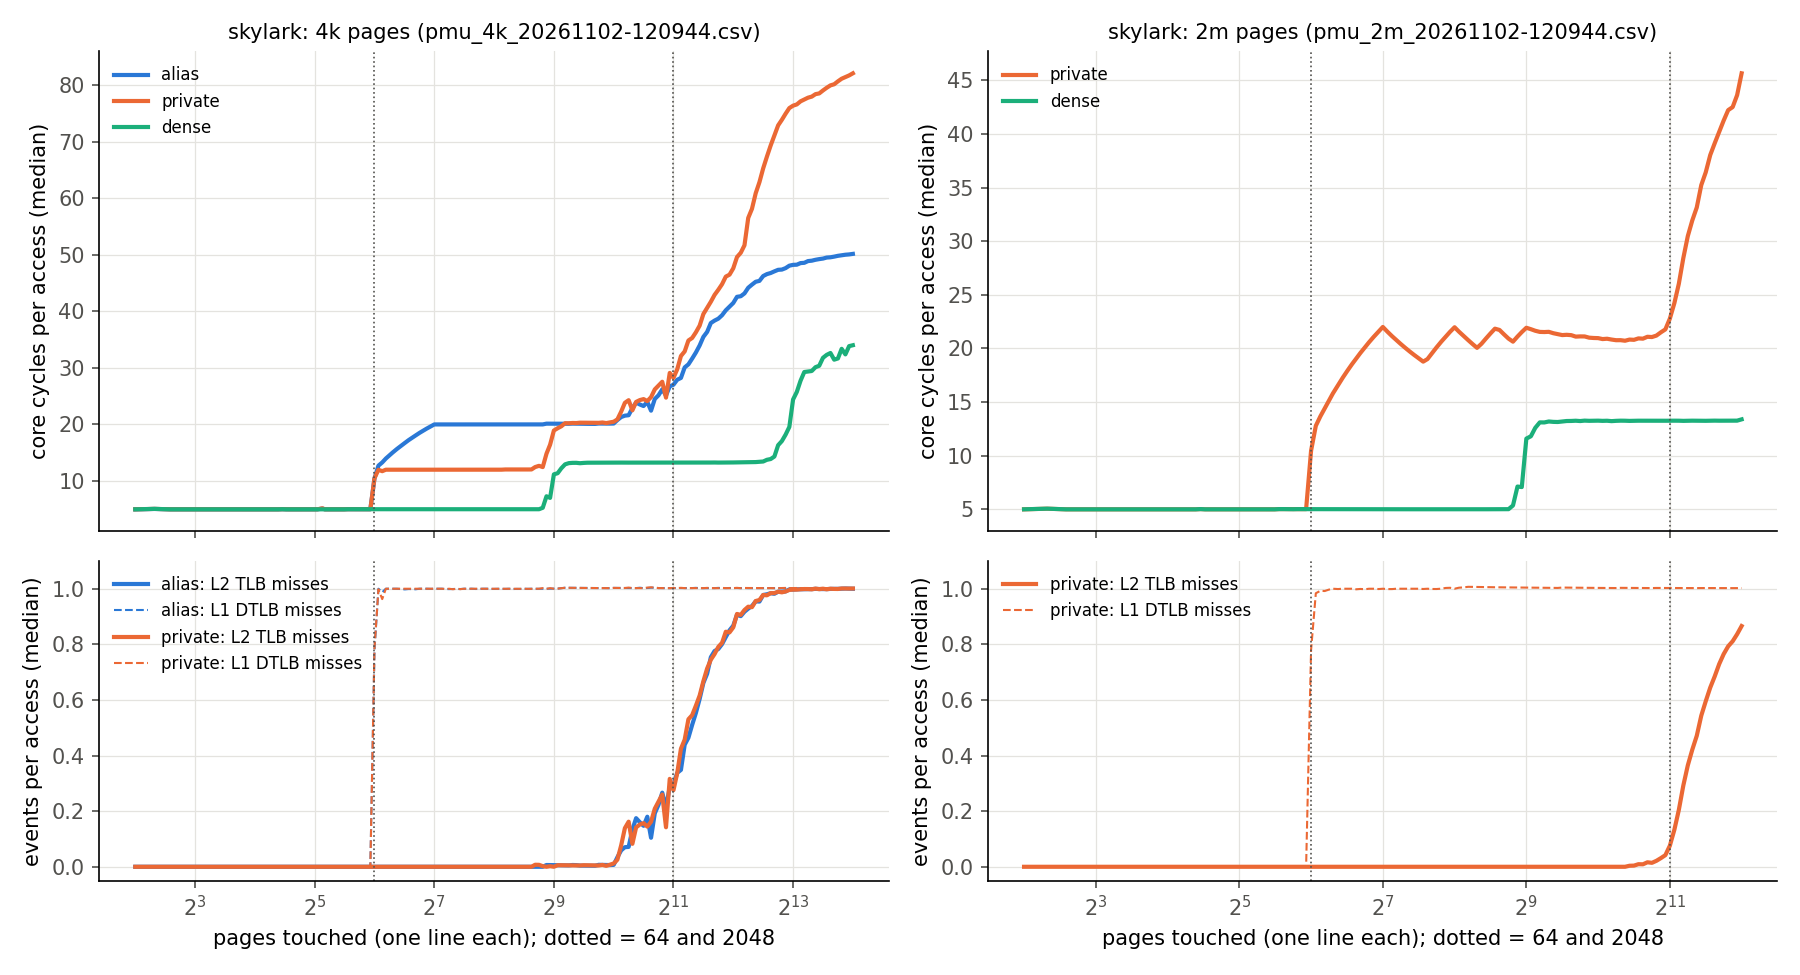
\includegraphics[width=\linewidth]{tlb_pmu.png}
\caption{\sk: core cycles per access (top) aligned with DTLB events per
access (bottom). Dotted lines mark the published Zen 2 capacities (64 and
2048) for reference.}
\label{fig:pmu}
\end{figure}

\begin{table}[h]
\centering
\small
\begin{tabularx}{\linewidth}{@{}lXX|l@{}}
\toprule
 & \multicolumn{2}{c|}{\textbf{Measured}} & \\
 & \up{} (timing) & \sk{} (timing + counters) & \textbf{Published} \\
\midrule
TLB levels & 2 & 2 & 2 on both \\
L1 DTLB, 4~KiB & 64: flat to 64, rises at 65 (both runs) & 0 misses at 62 pages, misses from 63 & CL: 64; Zen 2: 64 \\
L1 DTLB, 2~MiB & 32: flat to 32, rises at 33 (both runs) & identical to 4~KiB (0 at 62, misses from 63) & CL: 32; Zen 2: 64 (shared) \\
L2 TLB, 4~KiB & $\approx$1530 (extrapolates to 1529 and 1528) & no sharp edge: misses $>$1\% from $\approx$1024 pages, 50\% at 2435 & CL: 1536; Zen 2: 2048 \\
L2 TLB, 2~MiB & $\approx$1530 (extrapolates to 1531; run 1 only) & misses $>$1\% from 1408--1576, 50\% at 2704 & CL: 1536 (shared); Zen 2: 2048 \\
1~GiB pages & unavailable & unavailable & --- \\
\bottomrule
\end{tabularx}
\caption{Q6 and Q9: TLB levels and sizes. \up{} from two full runs, each
a coarse sweep plus dense refinements around each step (the second run's
2~MiB sweep is incomplete; see Repeatability); \sk{} from five sweeps per page size plus
refinements, and counter runs on both NUMA nodes. Published (CL = Coffee
Lake, which uses the Skylake core): Skylake~\cite{wc-skl,7cpu-skl}: L1 DTLB
4-way, STLB 12-way and holding both 4~KiB and 2~MiB entries; Zen
2~\cite{wc-zen2}: L1 DTLB fully associative for all page sizes, L2 TLB
holding 4~KiB and 2~MiB entries.}
\label{tab:tlb}
\end{table}

\begin{table}[h]
\centering
\small
\begin{tabular}{lcc|cc}
\toprule
 & \multicolumn{2}{c|}{\up{} (ns)} & \multicolumn{2}{c}{\sk{} (core cycles)} \\
 & 4~KiB & 2~MiB & 4~KiB & 2~MiB \\
\midrule
L1 TLB hit, total access cost & 1.37 & 1.34 & 5 & 5 \\
Added: L1 TLB miss, L2 TLB hit & +2.0 & +2.0 & +7.0 & +7.7 \\
Added: L2 TLB miss (page walk) & +3.0 & +3.5 & 25 at 4096 pages, 30 at 16384 & 27--28 at 4096 pages \\
\bottomrule
\end{tabular}
\caption{Q8: cost of TLB misses. \up{}: difference between plateau levels
(TSC ticks converted at 3.19 GHz); the second run gives +1.97 and +3.02~ns for 4~KiB. \sk{}: L2-hit cost from
\texttt{private} $-$ \texttt{dense}; page-walk cost as $\Delta$cycles $/$
$\Delta$(L2 misses per access) relative to 1024 pages, from the \texttt{alias}
curve (4~KiB) and \texttt{private} $-$ \texttt{dense} (2~MiB). At the
$\approx$1.49 GHz \sk{} clock, 7 cycles $\approx$ 4.7 ns and 25 cycles
$\approx$ 17 ns.}
\label{tab:q8}
\end{table}

\subsection{Interpretation}

\paragraph{Q6: two TLB levels on both machines.} Each machine shows exactly
two translation-caused steps before the cost keeps rising with page-walk
cache pressure. On \sk{} the counters confirm both: at 128 pages every
access is an L1 DTLB miss that hits the L2 TLB (1.00 per access, 0 L2
misses), and by 8192 pages every access is an L2 miss. The table-walk
counter equals the L2-miss counter (ratio 1.00), so every L2 TLB miss is
one page walk.

\paragraph{L1 DTLB size.} \up{} shows 64 entries for 4~KiB pages and 32 for
2~MiB. On \sk{}, 62 data pages fit with zero misses and misses begin at
63, for both page sizes. The chase loop also reads its \texttt{addrs[]}
array, which occupies one more page, so 63 entries are usable without
misses: one short of the published 64. Likely explanations are one entry
held by something else or the replacement policy; I did not separate them.

\paragraph{L2 TLB size.} On \up{} the L2 step is sharp and both page sizes
extrapolate to about 1530 entries, matching a published 1536-entry STLB
shared by 4~KiB and 2~MiB pages (both page sizes hit the same limit). On \sk{}
there is no sharp edge, and the counters show this is real, not a timing
artifact: with 4~KiB pages, L2 misses begin near 1024 pages (half the
published 2048) and reach 50\% only at 2435; 2~MiB pages begin later
(1408--1576) and reach 50\% at 2704. Page coalescing (Zen merging adjacent
4~KiB entries) is ruled out because the coalesced-page counter is 0
everywhere. A hashed set index that fills sets unevenly would produce this
shape; this is an untested hypothesis. The best supported statement is
that \sk{}'s L2 TLB holds on the order of 2048 entries, consistent with the
published size, but the capacity cannot be read off as a single step.

\paragraph{Q8: miss cost.} On \up, an L1 TLB miss that hits the STLB adds
about 2~ns per access and a page walk with cached page tables adds about
3--3.5~ns more. On \sk, an L2 TLB hit adds 7 cycles for 4~KiB and 7.7 for
2~MiB pages, and each page walk costs 25 cycles at 4096 pages, rising to 30
at 16384 as the page-table entries themselves stop fitting in the caches.

\paragraph{A confound found with the counters.} On \sk{}, the \texttt{alias}
pattern costs 20 cycles at 128 pages, and 2~MiB \texttt{private} costs 22,
against 12 for 4~KiB \texttt{private}, even though the counters show
identical TLB behavior (1 L1 miss, 0 L2 misses per access) and the data is
in L1. The extra cost is not additive: 2~MiB \texttt{private} costs 21
cycles at 1024 pages, where its data is in L2 anyway. This is consistent
with Zen's L1 data-cache way predictor (``$\mu$tag''), which is indexed by a
hash of the \emph{linear} address: \texttt{alias} reaches one physical line
through many linear addresses, and 2~MiB-strided slots that share an L1 set
differ only in high address bits. A mispredicted way makes an L1 hit cost
about as much as an L2 hit (13 cycles) plus the L2-TLB hit (7), i.e.\ 20.
This is a cache-side effect, not a TLB effect, which is why the Q8 L2-hit
costs on \sk{} are taken from \texttt{private} $-$ \texttt{dense} where it
cancels. It also means the \texttt{alias} pattern, the pure TLB signal on
Intel, is not pure on AMD.

\paragraph{Q9: page sizes.} Both machines support 4~KiB and 2~MiB pages to
user code; 1~GiB pages need a hugetlbfs pool that only root can reserve, and
neither machine has one. The organizations differ:
\begin{itemize}
\item \up{}: the L1 DTLB has separate capacities (64 for 4~KiB, 32 for
  2~MiB), while both sizes share one $\approx$1536-entry L2 TLB.
\item \sk{}: the L1 DTLB holds 64 entries of either size, and the L2 TLB
  favors 2~MiB entries slightly (misses begin about 300 pages later).
\end{itemize}
Huge pages increase reach by $512\times$: on \up{} the L2 TLB covers about
6~MiB with 4~KiB pages but about 3~GiB with 2~MiB pages; on \sk{} the L1
alone covers 256~KiB vs.\ 128~MiB. The cost of each kind of miss is
about the same for both page sizes on both machines (Table~\ref{tab:q8}).

\paragraph{Repeatability.} On \up{}, a second full run (Nov.~2) repeats
every ROB/PRF step within the sweep resolution of 4, and every 4~KiB TLB
result (L1 at 64, L2 extrapolating to 1528 vs.\ 1529, miss costs within
0.07~ns). Its 2~MiB sweep is not a valid repeat of the L2 step: memory was
fragmented, only 1513 of 2048 requested huge pages could be verified, and
the sweep stops below the L2 TLB. The verified pages also left gaps in the
virtual address range, and their L2 misses begin early (from about 1218
pages instead of about 1548), as expected if the L2 TLB set index comes
from virtual-address bits. The 2~MiB L1 result (32) does repeat. Figure~\ref{fig:tlb}
plots the most complete sweep for each page size.
On \sk{}, five coarse sweeps per page size (on
CPU~2 / NUMA node 0 and CPU~40 / node 1) agree within 0.5 cycles for the
4~KiB \texttt{alias} curve at every checked point from 56 to 16384 pages,
and within 1.6 cycles for 2~MiB at 4096 pages. 4~KiB \texttt{private} at
very large footprints is the exception (157 cycles at 16384 pages in one
run, 82 in two others), although each run is tight internally: physical
page placement changes how well data and page tables cache. This is a
cache effect, which is why page-walk costs use \texttt{alias}.

% ---------------------------------------------------------------------------
\section{Enclave comparison}
\label{sec:enclave}

The assignment asks for each experiment to be run inside and outside an
enclave on the same enclave-capable machine. Neither of the two main
machines can run one (Section~\ref{sec:noenclave}), so the comparison was
done on a third course machine, \texttt{artemisia}, which has Intel SGX
enabled. It is used only for this comparison; the two-machine results above
come from \up{} and \sk{}.

\subsection{Platform}

\begin{center}
\small
\begin{tabularx}{\linewidth}{@{}lX@{}}
\toprule
CPU & Intel Xeon Gold 5420+, Sapphire Rapids (Golden Cove cores), 2 $\times$ 28 cores, microcode \texttt{0x2b000685} \\
OS & RHEL 9.8, Linux 6.17.8, in-kernel SGX driver (\texttt{/dev/sgx\_enclave}), flexible launch control \\
EPC & two sections of about 1~GiB each \\
SGX software & Intel SGX SDK and PSW 2.23.100.2, hardware mode \\
Enclave & debug enclave signed with a locally generated key; 384~MiB heap; one thread \\
Runs & CPU~12 (its SMT sibling is offline); TSC 2.000~GHz; 4 rounds per mode \\
\bottomrule
\end{tabularx}
\end{center}

Gramine 1.6.2, which can run an unmodified binary inside an enclave, is also
installed, but its Python package (\texttt{graminelibos}) is missing, so its
manifest and signing tools fail. The comparison therefore uses the SDK
directly.

\subsection{Method}

The experiment code (\file{enclave/core.c}) is compiled twice from the same
source, with the same generated ROB/PRF kernels and the same TLB loop: into
an enclave, called through ECALLs, and into a normal process. Both builds use
4~KiB pages (enclave memory has no huge pages; the native build uses
\texttt{MADV\_NOHUGEPAGE}), the same buffer construction and the same random
seeds, so the only difference is whether the code runs inside the enclave.
Every call is timed from outside with the TSC in both modes, and the median
cost of an empty call is subtracted:

\begin{lstlisting}[language=C,caption={Timing one ROB measurement (\file{enclave/app.c}); \texttt{rob\_run} is an ECALL in the SGX build and a direct call in the native build.}]
uint64_t t0 = tsc_now();
rob_run(k, iters);                 /* 2000 loop iterations */
uint64_t t1 = tsc_now();
tsc_per_iter = (double)(t1 - t0 - ovh) / iters;   /* ovh: median empty call */
\end{lstlisting}

An ECALL round trip costs about 9{,}600 ticks (4.8~$\mu$s), against 42
ticks for a native call. Each timed call covers 0.6--1.4~M ticks (ROB) or at
least 400{,}000 loads (TLB), so the subtraction is a small correction.
Executing RDTSCP inside the enclave also works on this CPU (a separate
probe), unlike SGX1 processors where it faults; timing outside was kept so
both modes are measured identically.

What could not be done inside the enclave: 2~MiB pages (EPC has 4~KiB pages
only), so Q9's page-size comparison has no enclave counterpart; and the TLB
\texttt{alias} pattern (it maps one physical page many times through a
\texttt{memfd}), so the TLB signal is \texttt{private} $-$ \texttt{dense} in
both modes. perf counters were not used in either mode.

\subsection{Results}

\begin{figure}[h]
\centering
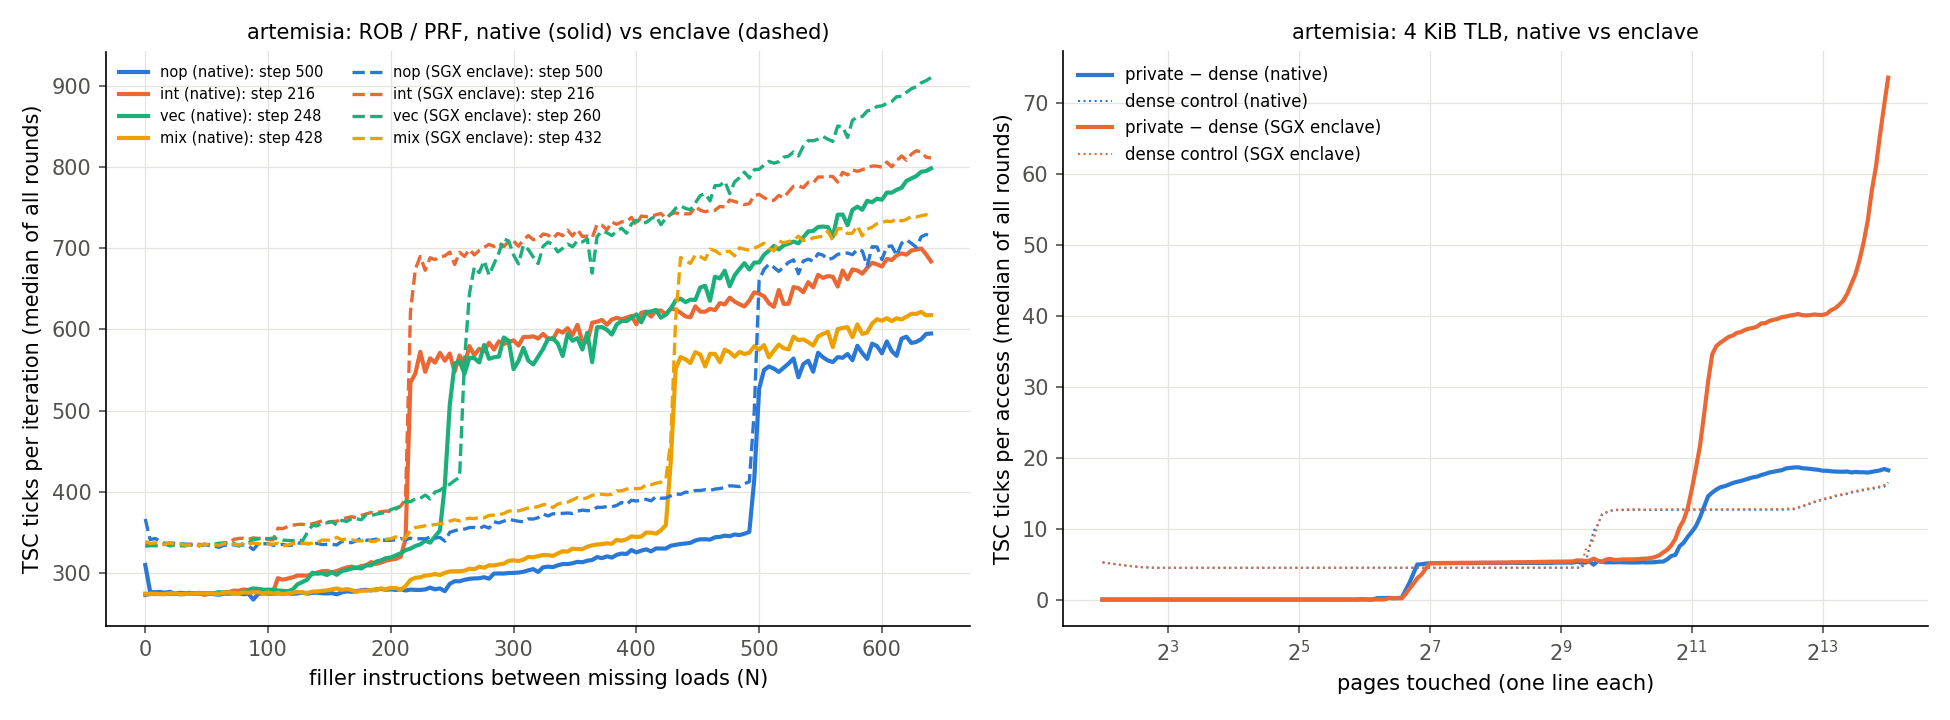
\includegraphics[width=\linewidth]{enclave.png}
\caption{\texttt{artemisia}: native (solid) vs.\ SGX enclave (dashed or
orange), medians of 4 rounds per mode. Left: ROB/PRF sweep. Right: TLB
translation cost (\texttt{private} $-$ \texttt{dense}) and the
\texttt{dense} cache-only control. Data: \file{data/artemisia/enclave/}.}
\label{fig:enclave}
\end{figure}

\begin{table}[h]
\centering
\small
\begin{tabular}{lcc|c}
\toprule
 & \multicolumn{2}{c|}{\textbf{Measured} (TSC ticks at 2.0~GHz)} & \textbf{Published} \\
 & Native & SGX enclave & Golden Cove \\
\midrule
\texttt{nop} step (ROB) & 496--500 & 496--500 & 512 \\
\texttt{add} step (integer PRF) & 216 & 216 & 280 \\
\texttt{addps} step (vector PRF) & 244--248 & \textbf{260} & 332 \\
alternating step & 428 & 432 & --- \\
ROB iteration, before / after the \texttt{nop} step & $\approx$276 / 560--590 & $\approx$340 / 690--705 & --- \\
L1 DTLB (refined knee) & 97 & 96 & 96 \\
L2 TLB onset (refined) & 1720--1744 & 1552--1576 & 2048$^\ast$ \\
L1 TLB miss, L2 TLB hit (128 pages) & +5.1 & +5.1 & +7 cycles \\
Beyond the L2 TLB, 4096 pages & 17.3 & \textbf{38.5} & --- \\
Beyond the L2 TLB, 16384 pages & 18.2 & \textbf{73.5} & --- \\
\bottomrule
\end{tabular}
\caption{Enclave comparison on \texttt{artemisia}. Step positions agree
across all 4 rounds in each mode within the sweep resolution of 4. The \texttt{dense} control is identical in
both modes at every point. Published: ROB~\cite{toms-gc,cnc-gc}, integer
PRF~\cite{cnc-spr-vrf}, vector PRF~\cite{wp-gc}, L1 DTLB~\cite{toms-gc},
L2 TLB hit cost~\cite{cnc-spr}; $^\ast$STLB size from a secondary
source only~\cite{blog-stlb}.}
\label{tab:enclave}
\end{table}

\subsection{Interpretation}

\begin{itemize}
\item \textbf{Core resources are unchanged inside the enclave.} The ROB
  step (about 500, against a published 512) and the integer register file
  step are identical in both modes, and so are the L1 DTLB size (96--97,
  published 96) and the cost of an L2 TLB hit.
\item \textbf{The alternating step supports separate register files.} It
  sits at 428--432 in both modes, well before the \texttt{nop} step. If each
  file receives half the demand, the integer file should run out at about
  $2 \times 216 = 432$, which matches.
\item \textbf{DRAM accesses are 20--22\% slower inside the enclave.} Both
  plateaus of the ROB curves rise (one and two memory latencies per
  iteration), consistent with SGX encrypting enclave memory on every cache
  miss. Cache hits are not slower: the \texttt{dense} control, which stays in
  the caches, is identical in both modes.
\item \textbf{Page walks are 2--4$\times$ more expensive inside the enclave},
  and the penalty grows with the number of pages touched (Figure~\ref{fig:enclave},
  right). Hits in either TLB level cost the same. This is consistent with
  SGX validating each new translation against the Enclave Page Cache Map
  (EPCM), whose entries must themselves be fetched and cached. The L2 TLB
  onset appears somewhat earlier inside the enclave, possibly because the
  more expensive walks make the first misses visible sooner; I did not test
  this.
\item \textbf{The vector register file step moves 16 later inside the
  enclave} (244--248 $\to$ 260) while the integer step does not. On Ice Lake
  server, touching any of the AVX-512 registers ZMM16--31 reserves 16 extra
  physical vector registers, and Golden Cove may behave the same
  way~\cite{cnc-spr-vrf}. A normal Linux process touches ZMM16--31 through
  glibc's AVX-512 string functions; the enclave code here never does, and
  enclave entry starts from clean extended register state. This explains
  the size of the shift, but I did not test it directly.
\end{itemize}

\subsection{Machines where an enclave run was not possible}
\label{sec:noenclave}

\begin{itemize}
\item \up{}: the i7-8700 supports SGX1 in hardware, but there is no
  \texttt{/dev/sgx\_enclave} or \texttt{/dev/isgx}, so SGX is not enabled in
  firmware or the kernel.
\item \sk{}: AMD processors do not implement SGX. AMD's closest feature,
  SEV, is present in the silicon (CPUID \texttt{0x8000001F} EAX =
  \texttt{0x1000f}: SME, SEV, SEV-ES), but the kernel reports
  ``SEV: memory encryption not enabled by BIOS'', and there is no
  \texttt{/dev/sev} or \texttt{/dev/kvm}. Enabling it requires
  administrator access to the BIOS. Even if enabled, SEV encrypts a whole
  virtual machine and needs KVM and root to launch one, so the comparison
  would be an encrypted VM vs.\ a plain VM rather than inside vs.\ outside an
  enclave within one process.
\end{itemize}

% ---------------------------------------------------------------------------
\section{Open questions and limitations}
\label{sec:open}

\begin{itemize}
\item \textbf{\sk{} integer PRF offset.} The integer step is 64 below the
  published size, compared with 36 on \up; the source of the extra
  integer-register demand on Zen 2 is not identified.
\item \textbf{\up{} integer and vector steps.} They fall at nearly the same
  $N$ (144--148), although the published sizes differ (180 and 168). I did
  not test whether two register files happen to run out together or a shared
  limit is responsible. A sweep that varies the integer-to-vector ratio could
  separate these.
\item \textbf{\up{} alternating step.} It falls about 12 below the
  \texttt{nop} step, and the cause is not identified.
\item \textbf{Shape of the ROB/PRF curves.} On both machines the cost drifts
  upward before the step and keeps rising after it. Front-end limits are a
  possible cause as the loop grows, but this was not tested.
\item \textbf{\texttt{artemisia} step offsets.} The steps sit further from the
  published sizes than on the other machines (about 500 vs.\ 512 for the ROB,
  216 vs.\ 280 integer, 244--260 vs.\ 332 vector). The sources of these gaps
  were not isolated.
\item \textbf{\sk{} L1 DTLB.} 63 entries are usable without misses against a
  published 64; the reason was not separated.
\item \textbf{\up{} 2~MiB L2 TLB.} The size comes from one run, because the
  second run's 2~MiB sweep was cut short by memory fragmentation.
\item \textbf{\sk{} L2 TLB shape.} The gradual miss curve is measured
  directly with counters, but the hashed-index explanation is untested. It
  could be tested by touching non-contiguous virtual pages.
\item \textbf{Way-predictor confound.} The explanation in
  Section~\ref{sec:tlb} fits the data, but Zen 2 exposes no event to confirm
  it, and cache reverse engineering is out of scope.
\item \textbf{No counters on \up{}.} Its TLB conclusions rest on timing
  alone, and its core clock during runs is unknown, so its results are in
  TSC ticks and ns.
\item \textbf{1 GiB pages} were unavailable on both machines
  (Section~\ref{sec:machines}).
\item \textbf{Enclave comparison.} It ran on a third machine (\texttt{artemisia}),
  in a debug enclave, for ROB/PRF and 4~KiB TLB only: 2~MiB pages and the
  \texttt{alias} pattern cannot exist in enclave memory. The vector-register,
  EPCM and L2-onset explanations in Section~\ref{sec:enclave} are not tested
  directly.
\end{itemize}

% ---------------------------------------------------------------------------
\appendix
\section{Submission contents and reproduction}
\label{app:repro}

\begin{center}
\small
\begin{tabularx}{\linewidth}{@{}lX@{}}
\toprule
Path & Contents \\
\midrule
\file{common/} & Shared helpers: TSC timing, CPU pinning, perf cycle and raw-event counters \\
\file{exp/rob_prf/} & Q4/Q5 kernel generator and sweep driver \\
\file{exp/tlb/} & Q6/Q8/Q9 timed loop and sweep driver \\
\file{scripts/} & \file{run_all.sh} (all experiments), \file{tlb_pmu.sh} (counter sweeps), \file{machine_info.sh} \\
\file{enclave/} & Enclave comparison: shared experiment core, ECALL interface, SGX and native drivers, \file{run_enclave.sh} \\
\file{analysis/} & Plotting and step-detection scripts; figures in \file{analysis/out/} \\
\file{data/<host>/} & Raw CSVs, run logs and \file{machine_info.txt} for each machine \\
\file{README.md} & Full reproduction instructions \\
\file{AI_LOG.md} & AI-use log (Track B) \\
\bottomrule
\end{tabularx}
\end{center}

To reproduce on an x86-64 Linux machine with gcc and Python 3 with
matplotlib:
\begin{lstlisting}[language=bash]
scripts/run_all.sh 2          # build, record machine info, run all sweeps on CPU 2
scripts/tlb_pmu.sh 2          # AMD only, needs perf: DTLB counter sweeps
python3 analysis/plot_rob_prf.py && python3 analysis/plot_tlb.py
python3 analysis/plot_tlb_pmu.py
enclave/run_enclave.sh 12 2   # SGX machine with the Intel SGX SDK: enclave vs native
python3 analysis/plot_enclave.py
\end{lstlisting}

\paragraph{AI use.} This work was done under Track B with AI assistance
(Claude, via Claude Code), as detailed in \file{AI_LOG.md}.

% Published specifications only; every measured value in this report comes
% from the experiments. Checked 2026-11-02.
\begin{thebibliography}{9}
\small
\bibitem{wc-skl} WikiChip, ``Skylake (client) -- Microarchitectures -- Intel.''
  \url{https://en.wikichip.org/wiki/intel/microarchitectures/skylake_(client)}
  (ROB 224; integer PRF 180; L1 DTLB 64/32/4 entries for 4~KiB/2~MiB/1~GiB, 4-way;
  STLB 1536 entries, 12-way, 4~KiB and 2~MiB).
\bibitem{7cpu-skl} 7-cpu.com, ``Intel Skylake.''
  \url{https://www.7-cpu.com/cpu/Skylake.html} (same TLB sizes and associativity).
\bibitem{arxiv-skx} R.~Sch\"one, T.~Ilsche, M.~Bielert, A.~Gocht, D.~Hackenberg,
  ``Energy Efficiency Features of the Intel Skylake-SP Processor and Their
  Impact on Performance,'' arXiv:1905.12468, 2019 (ROB 224; integer PRF 180;
  FP PRF 168; Skylake-SP uses the same core).
\bibitem{wp-snc} Wikipedia, ``Sunny Cove (microarchitecture)''
  (vector register file 224 entries, ``up from 168'' in Skylake).
\bibitem{wc-zen2} WikiChip, ``Zen 2 -- Microarchitectures -- AMD.''
  \url{https://en.wikichip.org/wiki/amd/microarchitectures/zen_2}
  (retire queue 224; integer PRF 180; FP PRF 160; L1 DTLB 64 entries, fully
  associative, 4~KiB/2~MiB/1~GiB; L2 DTLB 2048 entries, 4~KiB and 2~MiB, 1~GiB
  pages smashed to 2~MiB).
\bibitem{toms-gc} Tom's Hardware, ``Intel Architecture Day 2021: Golden Cove,''
  \url{https://www.tomshardware.com/features/intel-architecture-day-2021-intel-unveils-alder-lake-golden-cove-and-gracemont-cores/4}
  (ROB 512; L1 DTLB 96 entries).
\bibitem{cnc-gc} C.~Lam, ``Popping the Hood on Golden Cove,'' Chips and Cheese, 2021,
  \url{https://chipsandcheese.com/p/popping-the-hood-on-golden-cove} (ROB 512).
\bibitem{wp-gc} Wikipedia, ``Golden Cove'' (vector register file 332 entries).
\bibitem{cnc-spr-vrf} Chips and Cheese, ``Golden Cove's Vector Register File:
  Checking with Official (SPR) Data,''
  \url{https://chipsandcheese.com/p/golden-coves-vector-register-file-checking-with-official-spr-data}
  (integer register file 280, 288 per SPR slides; on Ice Lake server, touching
  ZMM16--31 reserves 16 extra vector registers).
\bibitem{cnc-spr} Chips and Cheese, ``Sapphire Rapids: Golden Cove Hits Servers,'' 2023,
  \url{https://chipsandcheese.com/2023/03/12/a-peek-at-sapphire-rapids/}
  (L2 TLB hit adds 7 cycles).
\bibitem{blog-stlb} junxnone, ``Mem TLB,''
  \url{https://github.com/junxnone/opt/issues/73} (Sapphire Rapids STLB 2048
  entries, attributed to Intel's optimization manual; not verified there).
\end{thebibliography}

\end{document}
